\documentclass{article}
\usepackage[utf8]{inputenc}
\usepackage[margin=1in]{geometry}
\usepackage{graphicx}
\usepackage{amsmath,amscd}
\usepackage{amssymb}
\usepackage{mathptmx}

\title{Safe Vertex Connection Method Between Different Layers Based on Heuristic KC, 2D Case}
\author{Sipu Ruan \thanks{ruansp@jhu.edu}}

\begin{document}
\maketitle

\begin{enumerate}
\item {\bf General Ideas}\\
We encapsulate the actual elliptical robot with a larger ellipse, and do the Minkowski operations between the larger one and the environment. Then the smaller ellipse can have some free motions inside the larger one. As a result, for each vertex generated in previous steps, the smaller ellipse has a ``local c-space'' for free motions. To determine whether two vertices in different layers can be safely connected, we look into their ``local c-space'', as shown in fig \ref{fig:c-space} and fig \ref{fig:c-space-fitted}. The condition for connectivity is that the two local c-space should have an intersection area, from where we could find another vertex, denoted ``middle vertex'', to connect both of them safely.

\begin{figure}[h]
\centering
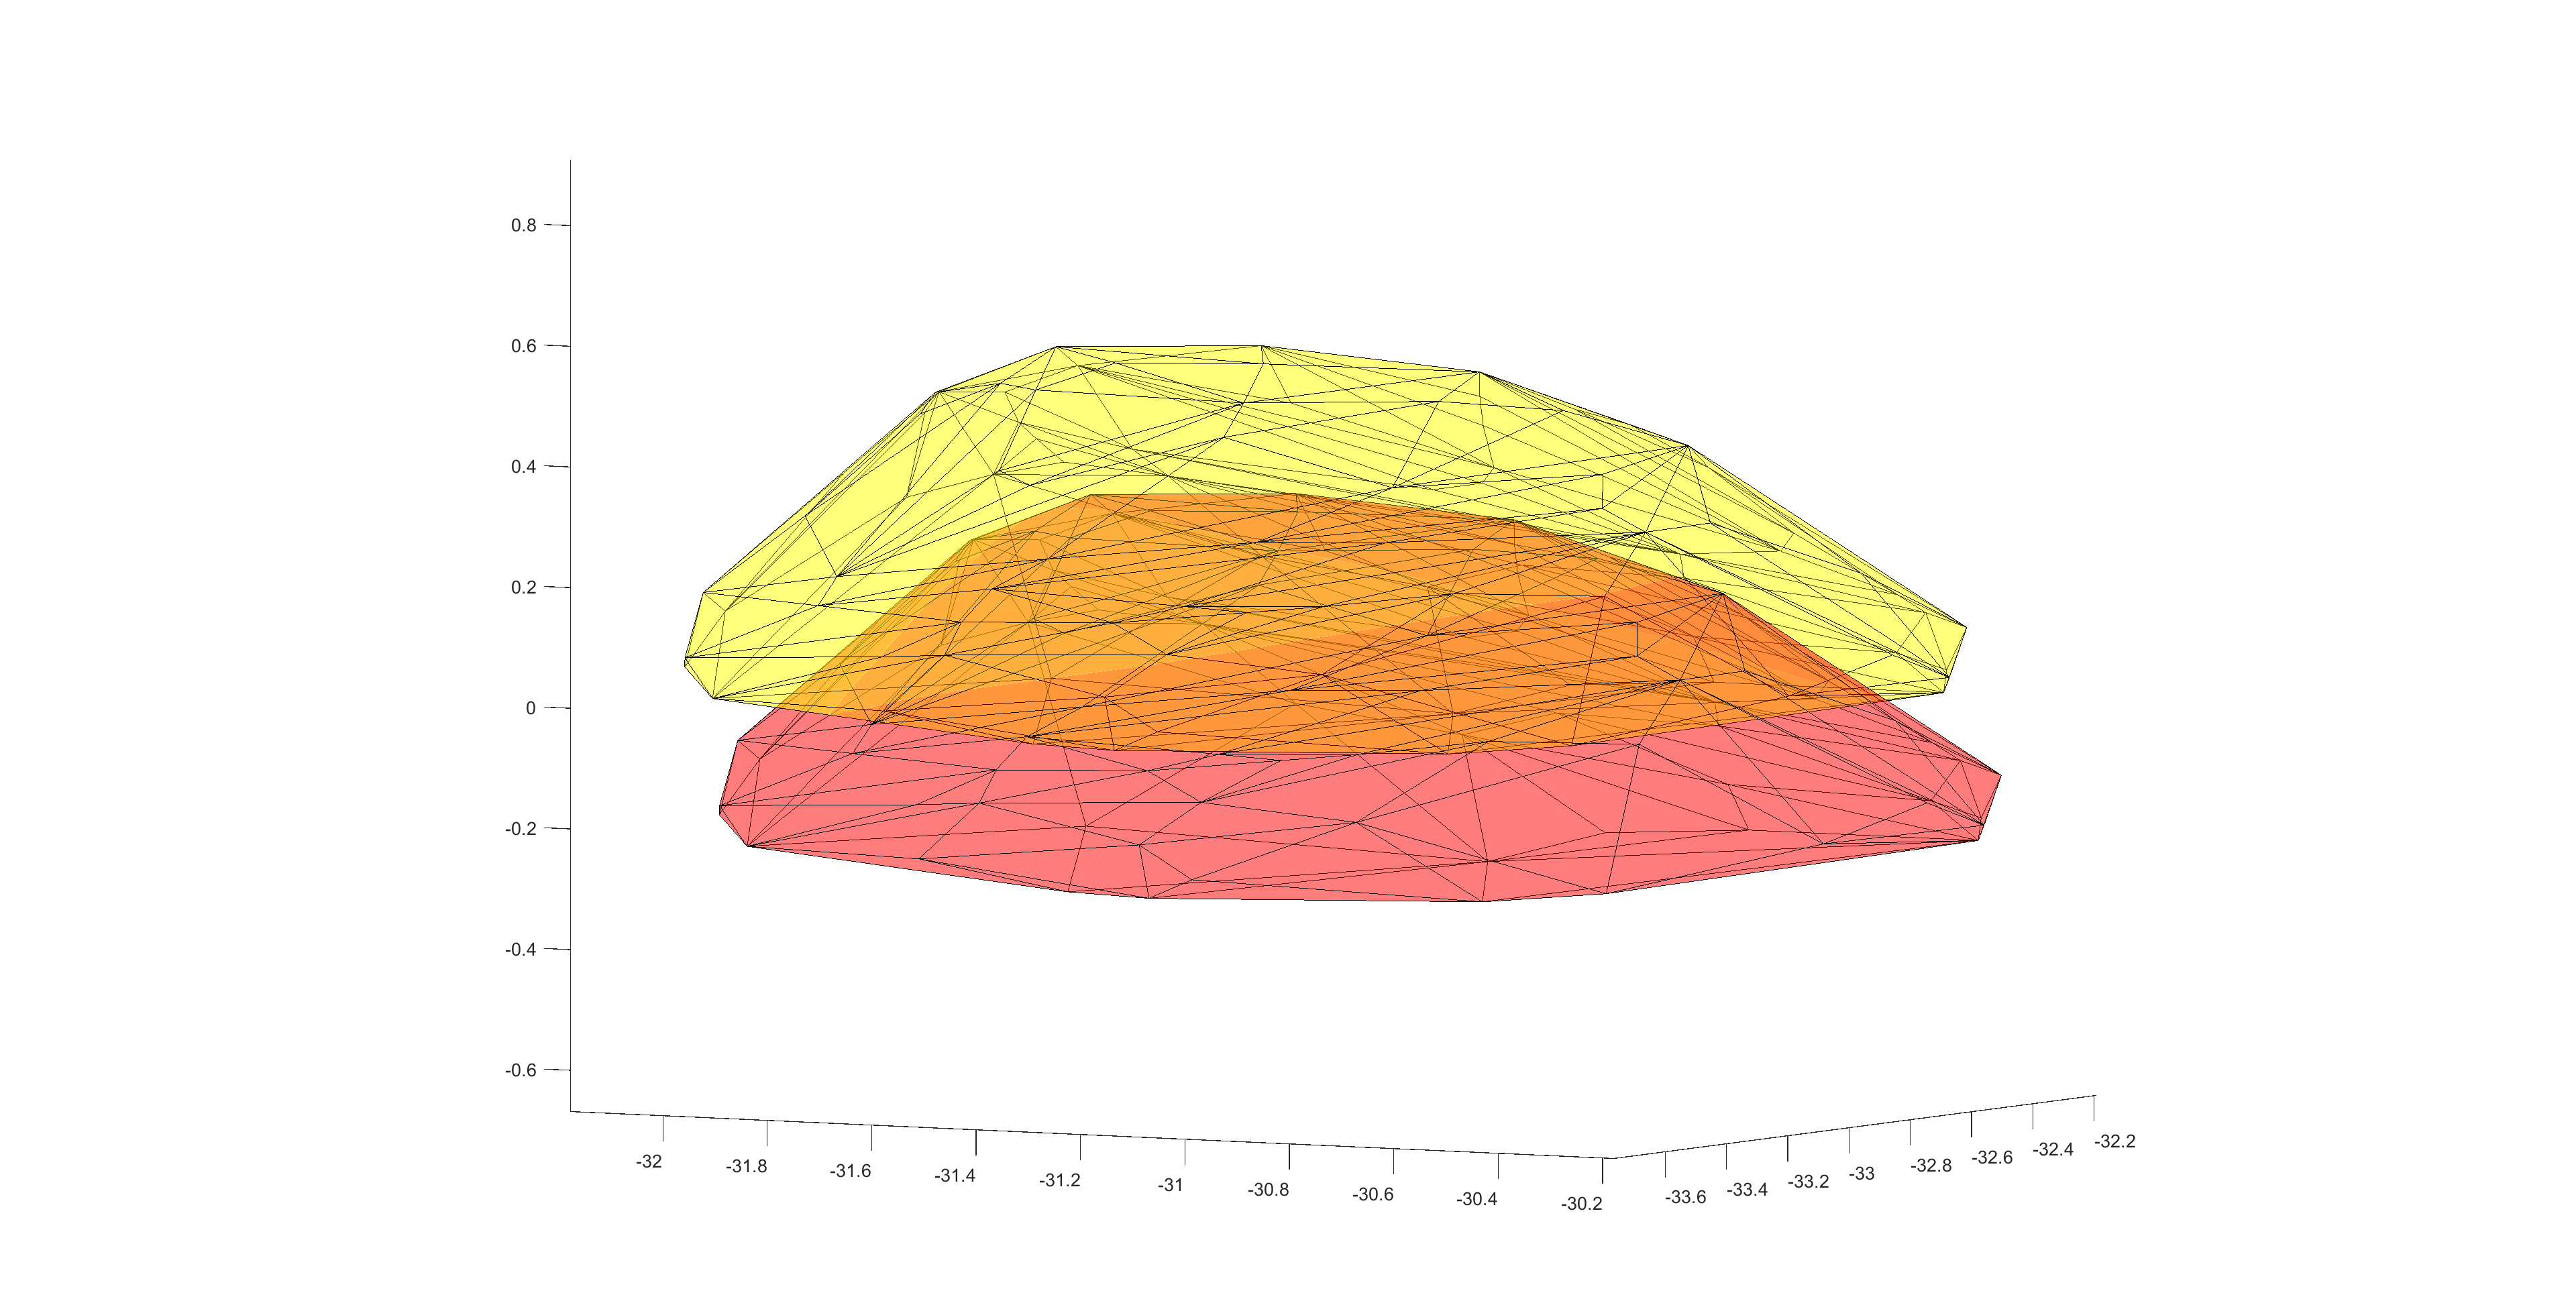
\includegraphics[scale=0.1]{layer_connection_c-space.png}
\caption{Sample-based local c-space for two vertices}
\label{fig:c-space}
\end{figure}
\begin{figure}[h]
\centering
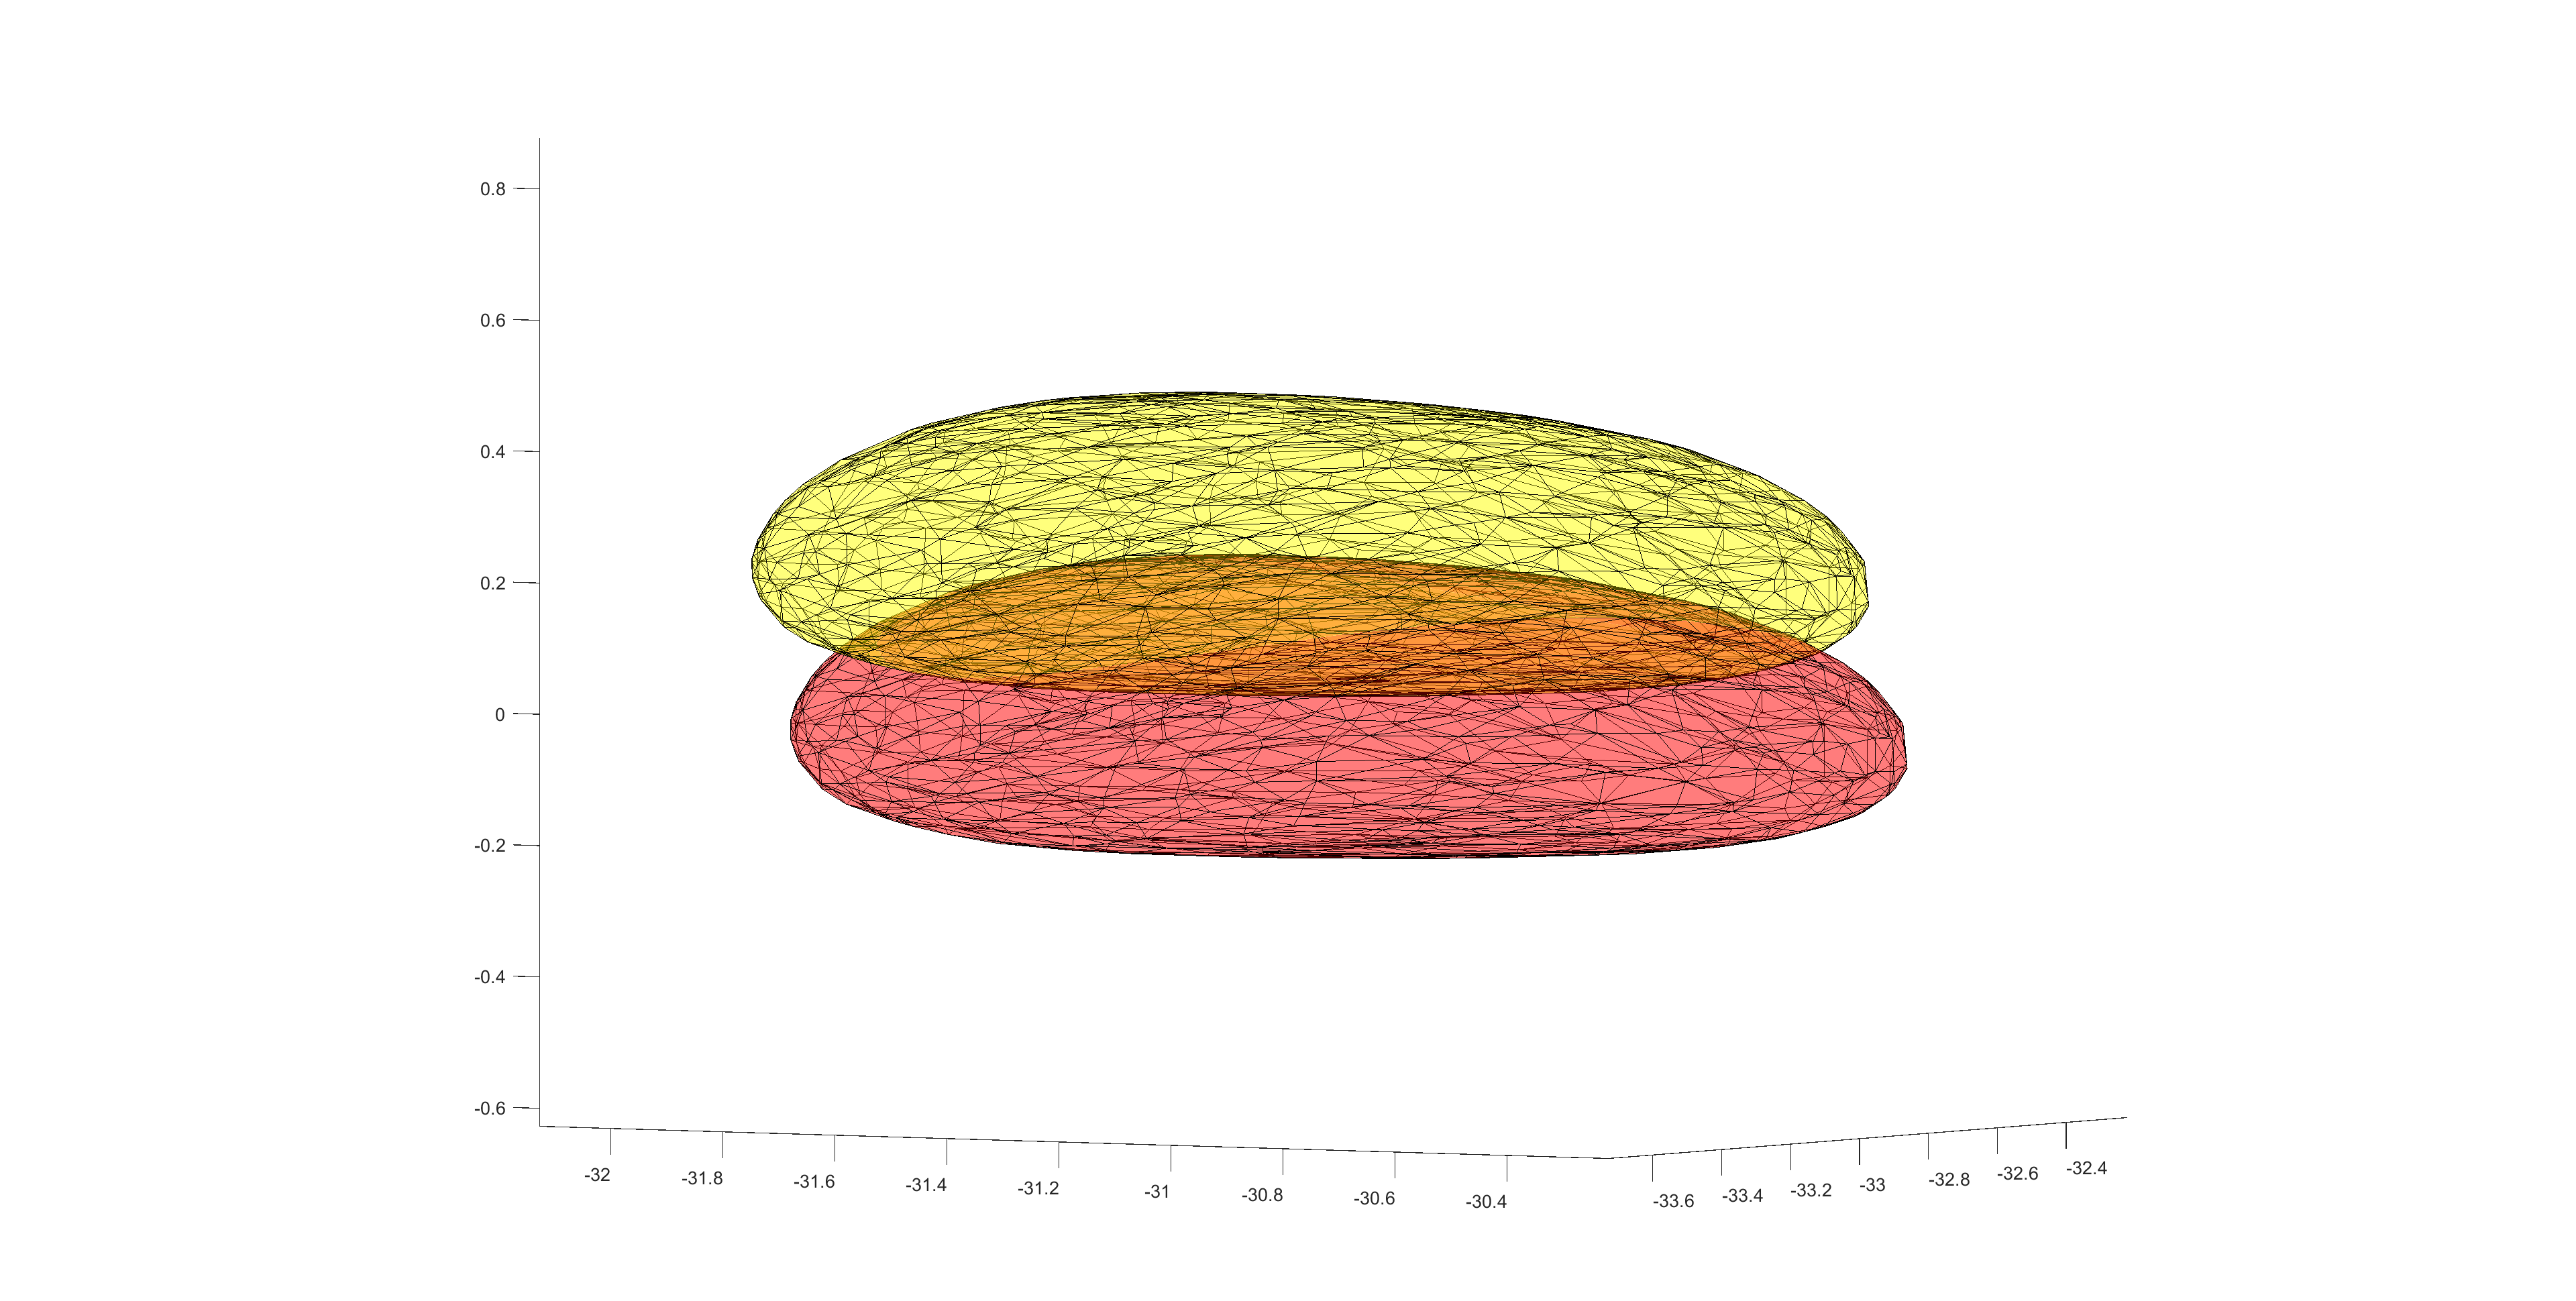
\includegraphics[scale=0.1]{layer_connection_c-space_fitted.png}
\caption{``twisted ellipsoid'' local c-space for two vertices}
\label{fig:c-space-fitted}
\end{figure}

We generate the local c-space by using Kinematics of Containment (KC) method, which will be stated below. Since the exact KC is hard to find, we propose two methods to approximate: Twisted Ellipsoid Fit and Polyhedron Fit, each of which has advantages and limitations, but can be pre-proceeded and queried quickly.

\item {\bf Implementation details}\\
\begin{enumerate}
\item {\bf Pre-proceed the local c-space}\\
Since the shape of the robot is fixed, the local c-space for free motion in the local frame of each vertex is the same. So we could generate the local c-space at the beginning of the motion planning process and treat it as a priori. When checking for the connectivity, we could only add an offset for each vertex to get the local c-space in global frame. The details of generating heuristic KC volume are describe in ``HeuristicKC'' file.

\item {\bf Find the middle vertex}\\
Generally speaking, we could generate local c-space in all vertices, but in practice, we only deal with the case when the two vertices, which are in adjacent layers, have a relatively close Euclidean distance to eliminate unnecessary calculations. If the two vertices are close to each other, we generate their local c-space, and find a middle vertex in the intersection area. 

To determine whether two vertices are close, we do a scan through the vertices in both layers in almost linear time complexity as follows. When we store the vertices, we already sorted them in ascending order according to angles, y coordinates and x coordinates successively. When querying, we go through the list of vertices in layer $i$ first, and traverse through the list of vertices in layer $i+1$. Once we find a vertex in list $i+1$ that is close to vertex in layer $i$, we access the local c-space and find middle vertex in their intersection. Then, the index of the vertex in list $i+1$ is recorded, and so we could start from this vertex in layer $i+1$ to search for the closest vertex with the next vertex in layer $i$ in the following iteration. After such iterative process is done, both lists are accessed only once, thus the complexity can be considered as $O(N)$.

To query if a vertex is inside the intersection of two local c-space, we could do a ``sample-test'' procedure to find if a candidate vertex is inside of both local c-space. For each approximation, we proposed a procedure to find points inside the intersection of two volumes.

\begin{enumerate}
\item {\bf Intersection of two ``twisted ellipsoids''}\\
For the twisted ellipsoid case, we do this by randomly sample a configuration within the range of the untwisted ellipsoidal local c-space of Vertex 1 (on the local frame of Vertex 1), and check if it is inside the ellipsoid. If so, we twist the space and transform into the global frame, so we get the global coordinate of the sampled point. Now we check if the point is inside the local c-space of Vertex 2 by transforming the point to the locally untwisted space of Vertex 2, and check if it is inside the untwisted ellipsoid. If so, we record the global coordinate of the point. We do the process iteratively until a valid sample is found or the maximum number of samples is reached, for which case the two vertices cannot be connected. Fig \ref{fig:c-space-fitted-midVtx} shows the sampled points in the intersection area of the two local c-space. 

\begin{figure}[!h]
\centering
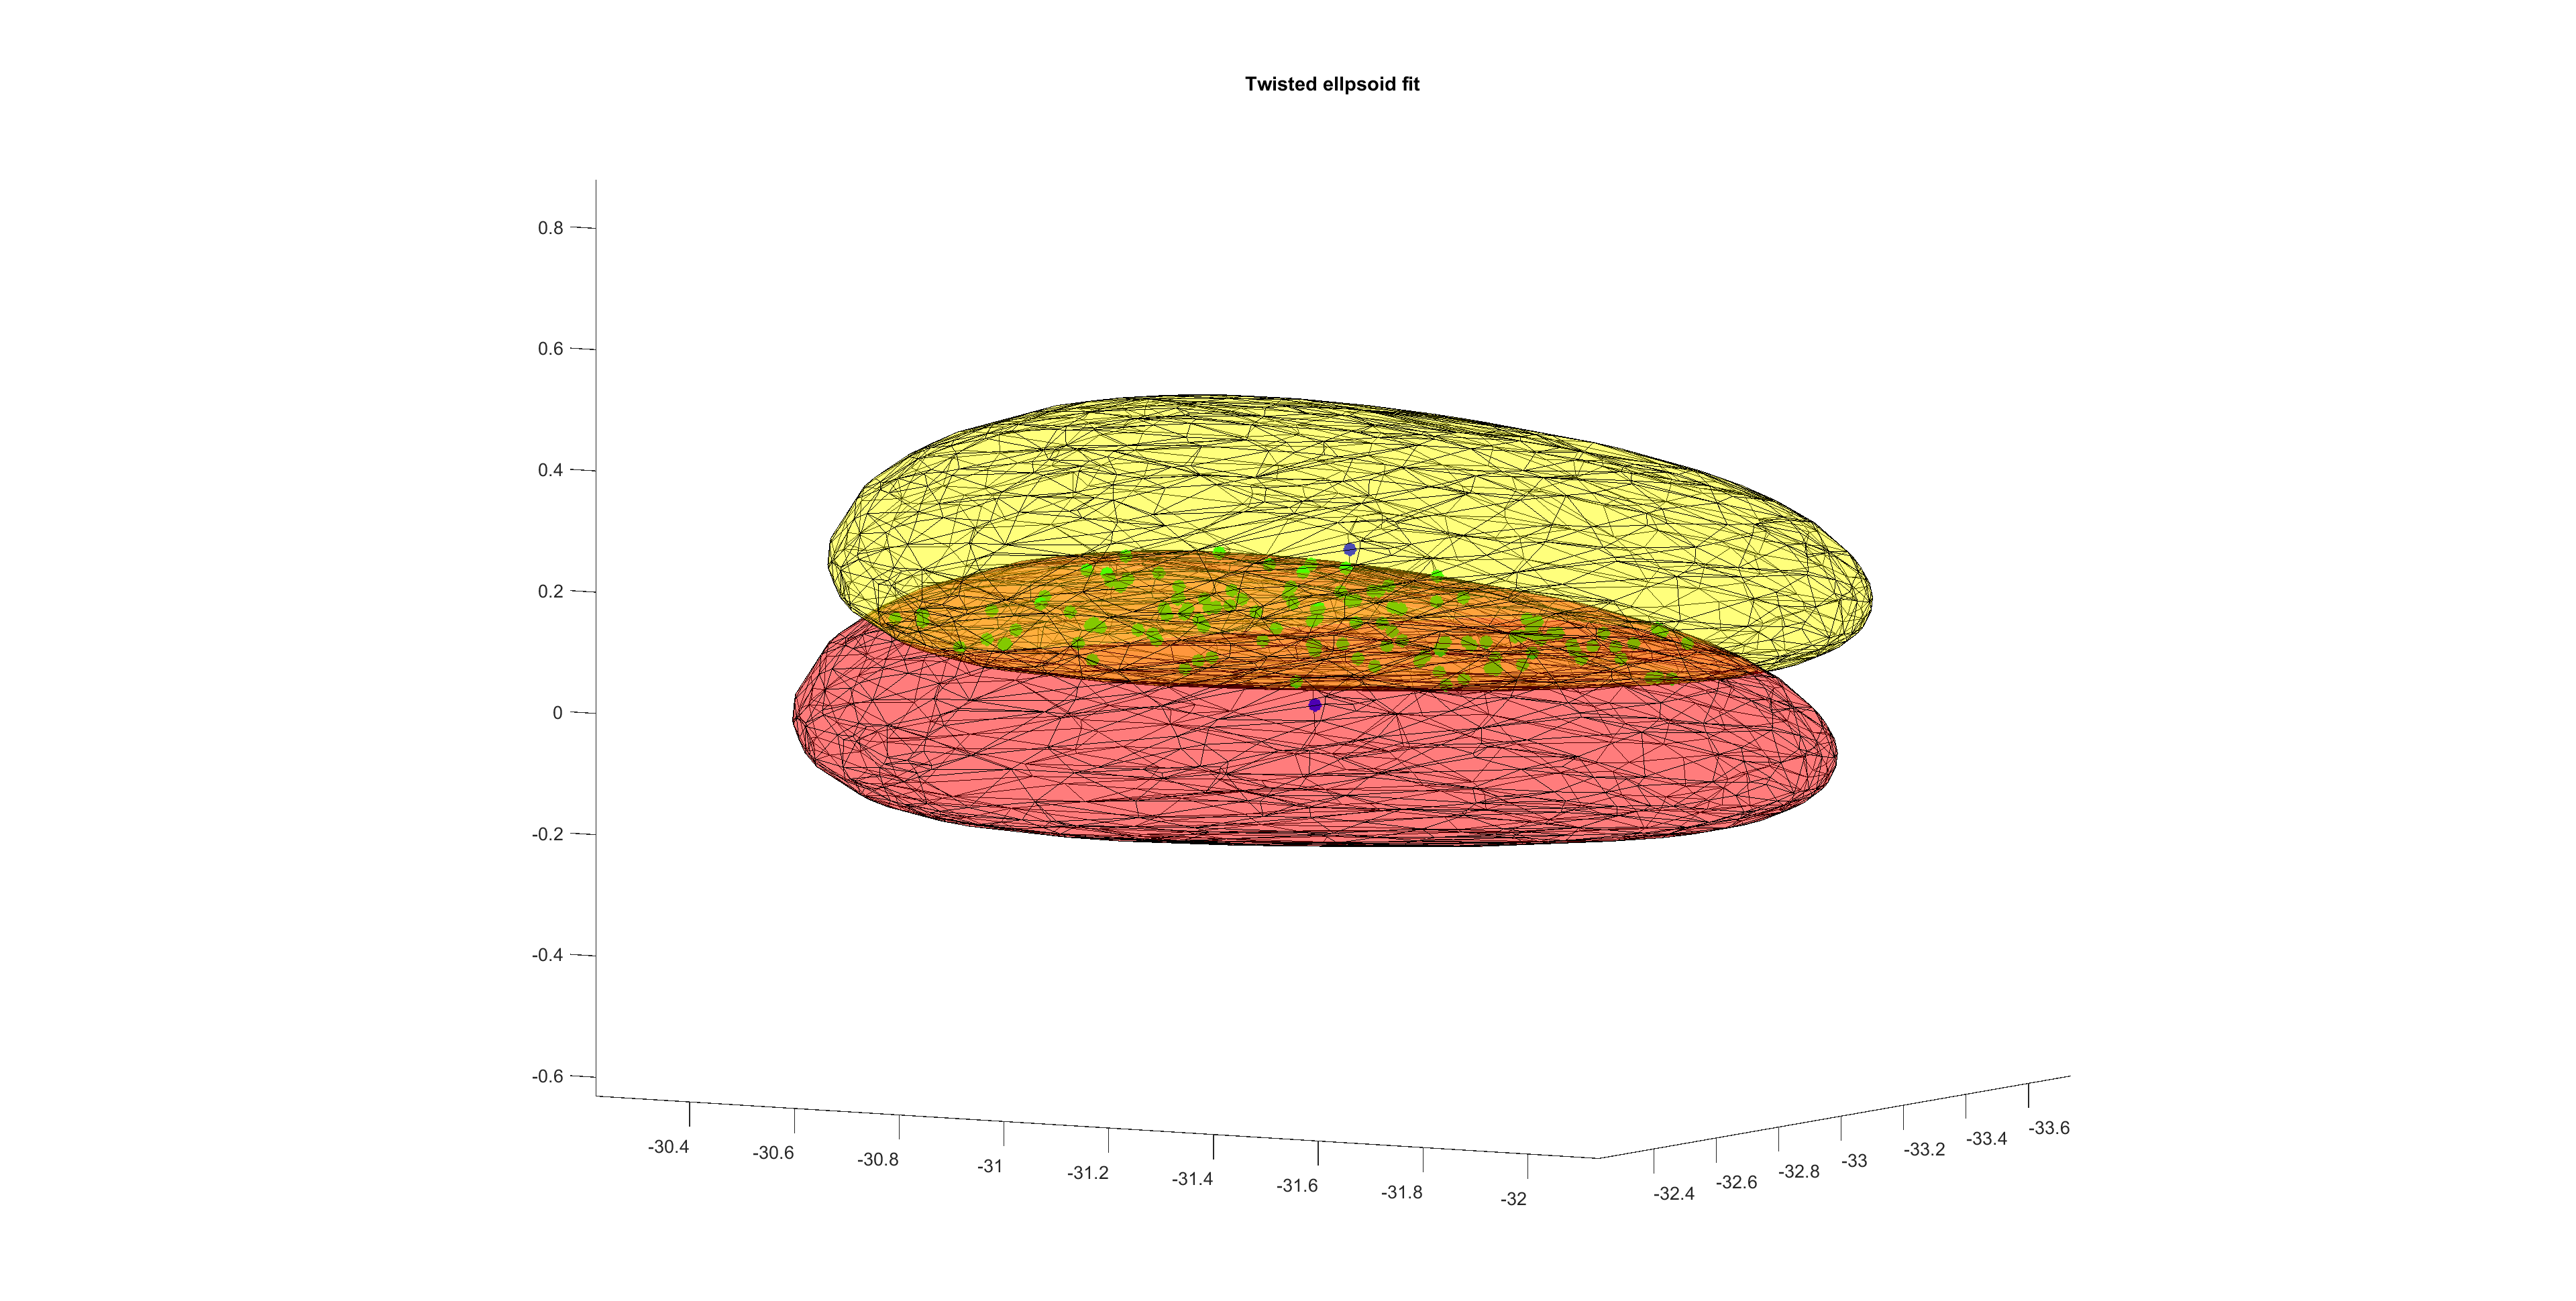
\includegraphics[scale=0.15]{layer_connection_c-space_fitted_midVtx.png}
\caption{Sampled points in intersection (green), vertices (blue)}
\label{fig:c-space-fitted-midVtx}
\end{figure}

To further speed up the testing process, after a point is sampled, we could locate the section plane, which is vertical the twisting axis, that the point is in. Since the section of a twisted ellipsoid is an ellipse, the intersection problem becomes testing a point inside the intersection of two ellipses, which could reduce the computation complexity. Fig \ref{fig:c-space-fitted-midVtx-ellipse-inter} demonstrates the idea.

\begin{figure}[!h]
\centering
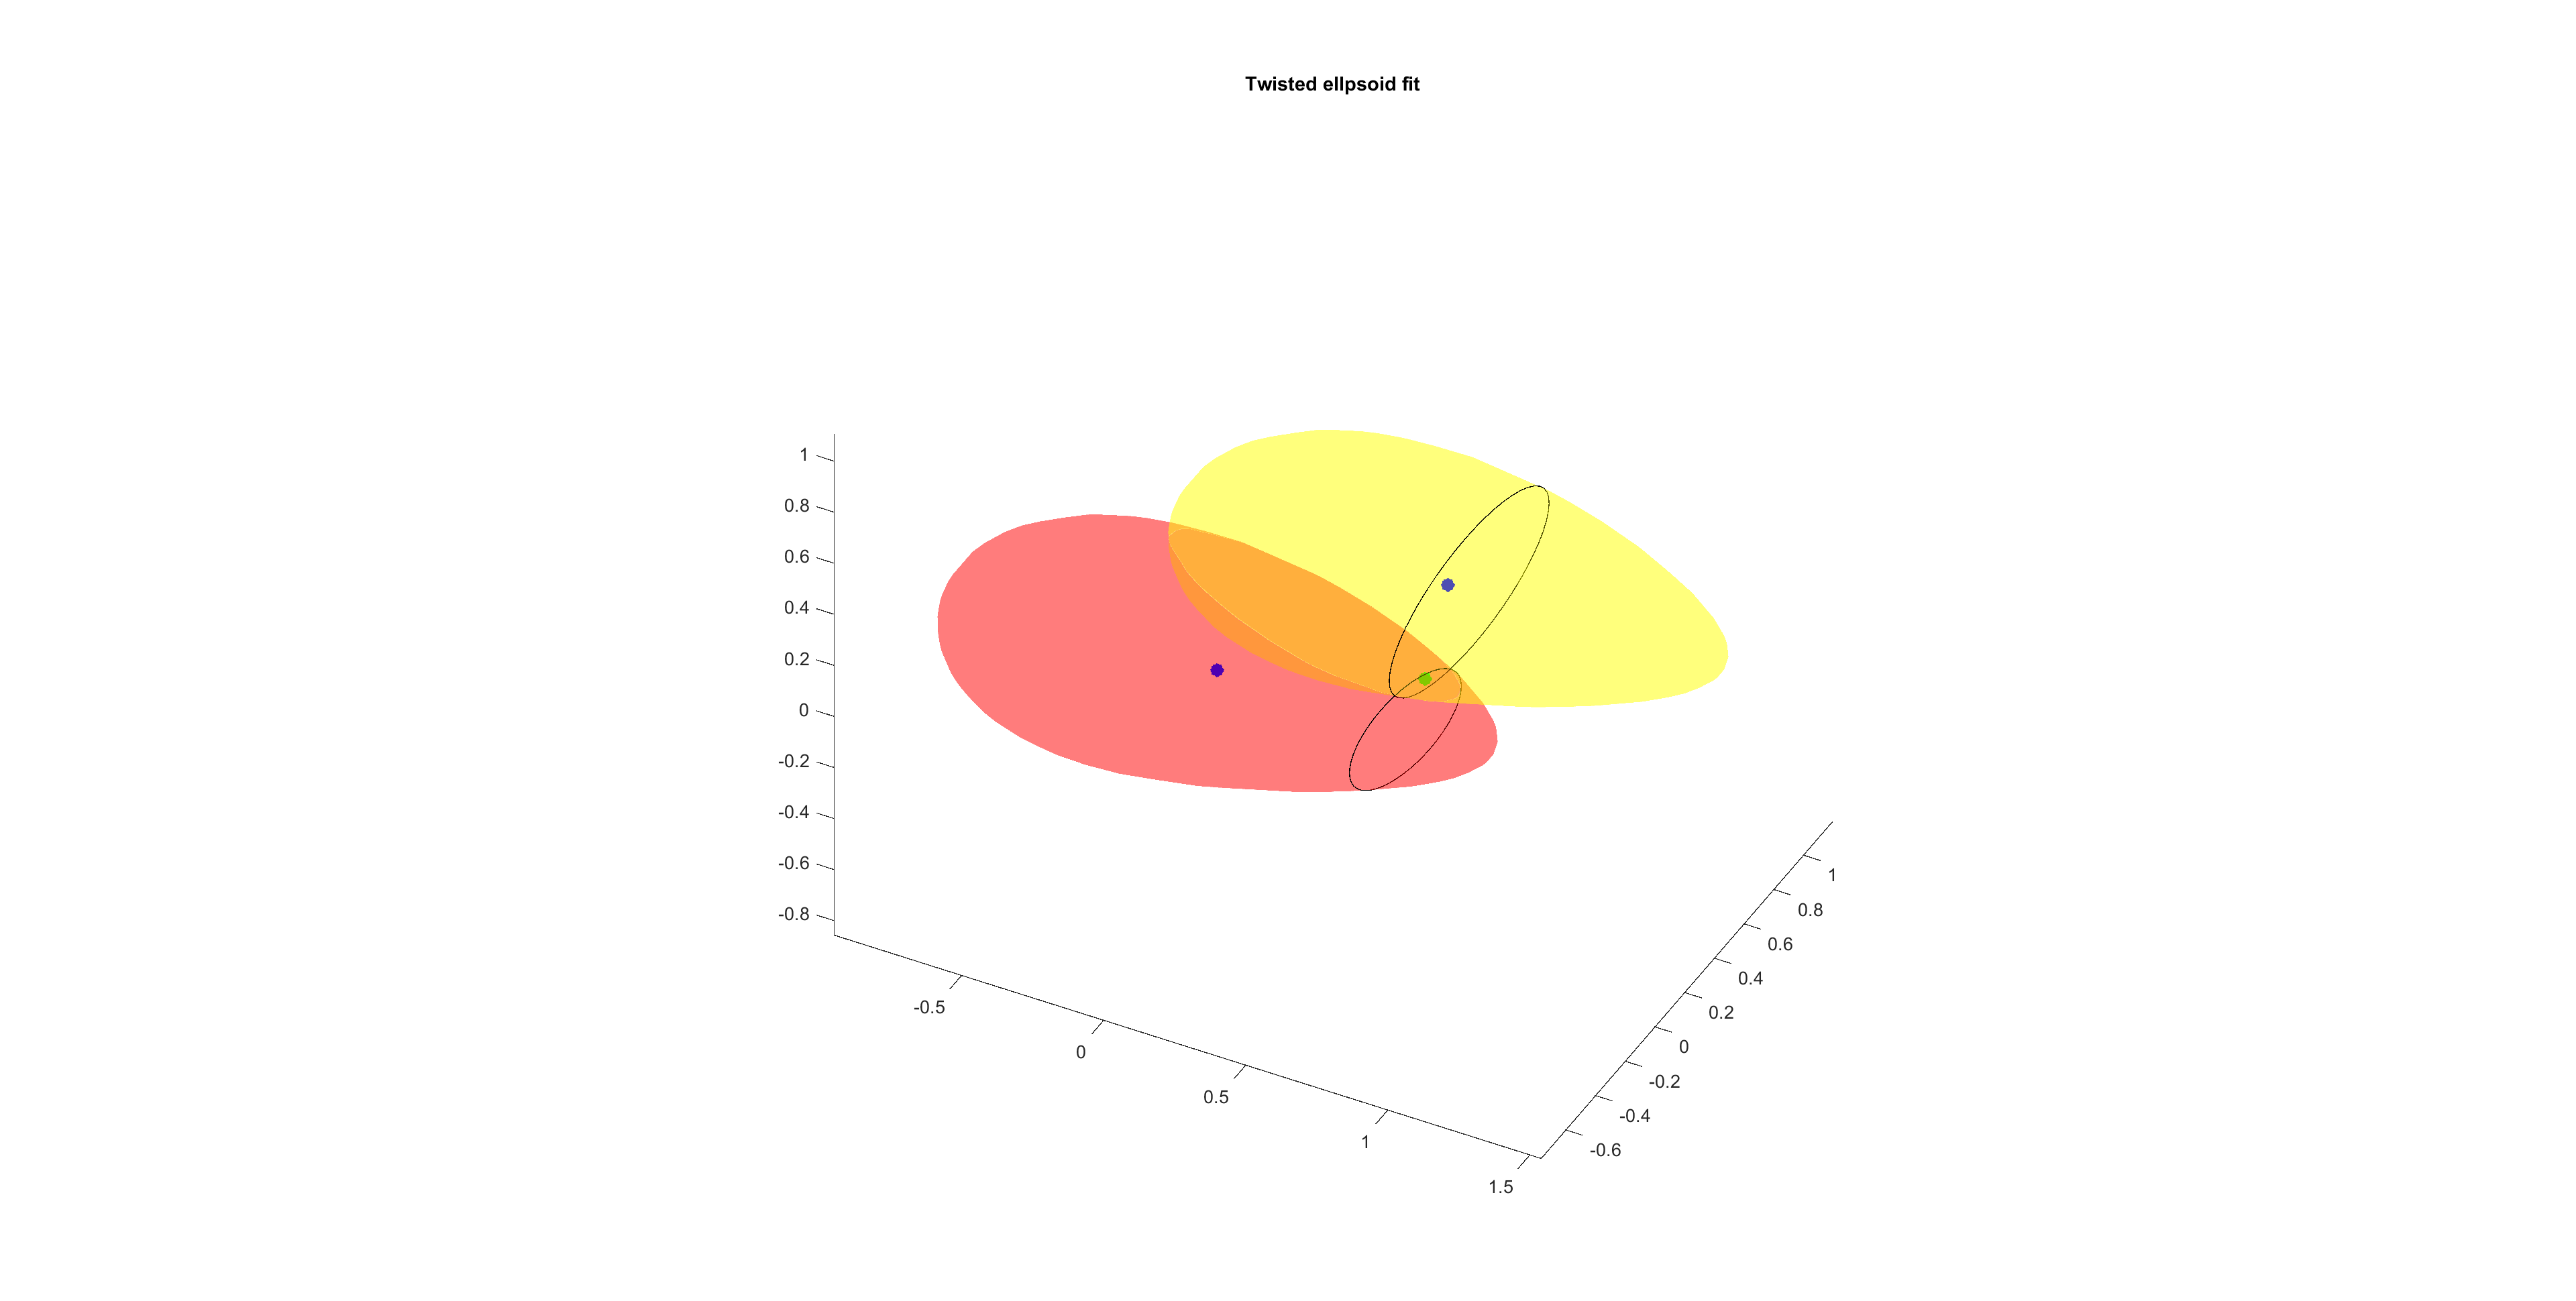
\includegraphics[scale=0.15]{Sample-based_middle_point_test_demo.png}
\caption{Sampled point in intersection of the section plane of two twisted ellipsoids}
\label{fig:c-space-fitted-midVtx-ellipse-inter}
\end{figure}

\item {\bf Intersection of two polyhedra}\\
Testing a point inside the intersection of two polyhedra requires simply testing if the point is in the interior of both volumes. There are many methods to determine a point inside a polyhedron, for our case in particular, where the number of vertices is small, we first decompose the shape into a union of simplexes, i.e. tetrahedron in 3D case, and check whether the point can be written as a convex combination of vertices of the simplex.

We use Delaunay triangulation to get the union of simplexes, and the point-in-simplex test can be done by constructing a linear system of equations as follows. The convex combination of 4 vertices can be expressed as $x = \sum_{i=1}^{4} \alpha_i v_i$ where $\alpha_i \in [0,1], \sum_{i=1}^{4} \alpha_i = 1$. Grouping into homogeneous matrix form gives
\begin{equation}
\left( \begin{matrix} v_1 & v_2 & v_3 & v_4\\ 1 & 1 & 1 & 1 \end{matrix} \right) 
\left( \begin{matrix} \alpha_1 \\ \alpha_2 \\ \alpha_3 \\ \alpha_4 \end{matrix}\right) = \left(\begin{matrix} x \\ 1 \end{matrix}\right)
\text{    where,  } \sum_{i=1}^{4} \alpha_1 = 1
\end{equation}

The problem becomes solving such linear system of equations given $v_i, i = 1...4$ and $x$, which can be done by inverting the matrix of vertices and testing if $\alpha_i \in [0,1], i = 1...4$. Note that the matrix of vertices is invertible if the 4 vertices are not located on the same plane or the same line.

Such procedure can be expanded if we need to test many points, in which case we just form a matrix of testing points on the right hand side and solve the new system of equations. Then, for each column of the result, we do the range test for all elements in that column. By this means can we test by solving the linear system of equations once, rather than calculating iteratively. Fig \ref{fig:c-space-fitted-midVtx-poly} demonstrates the vertex connection scheme using polyhedron fit.

\begin{figure}[!h]
\centering
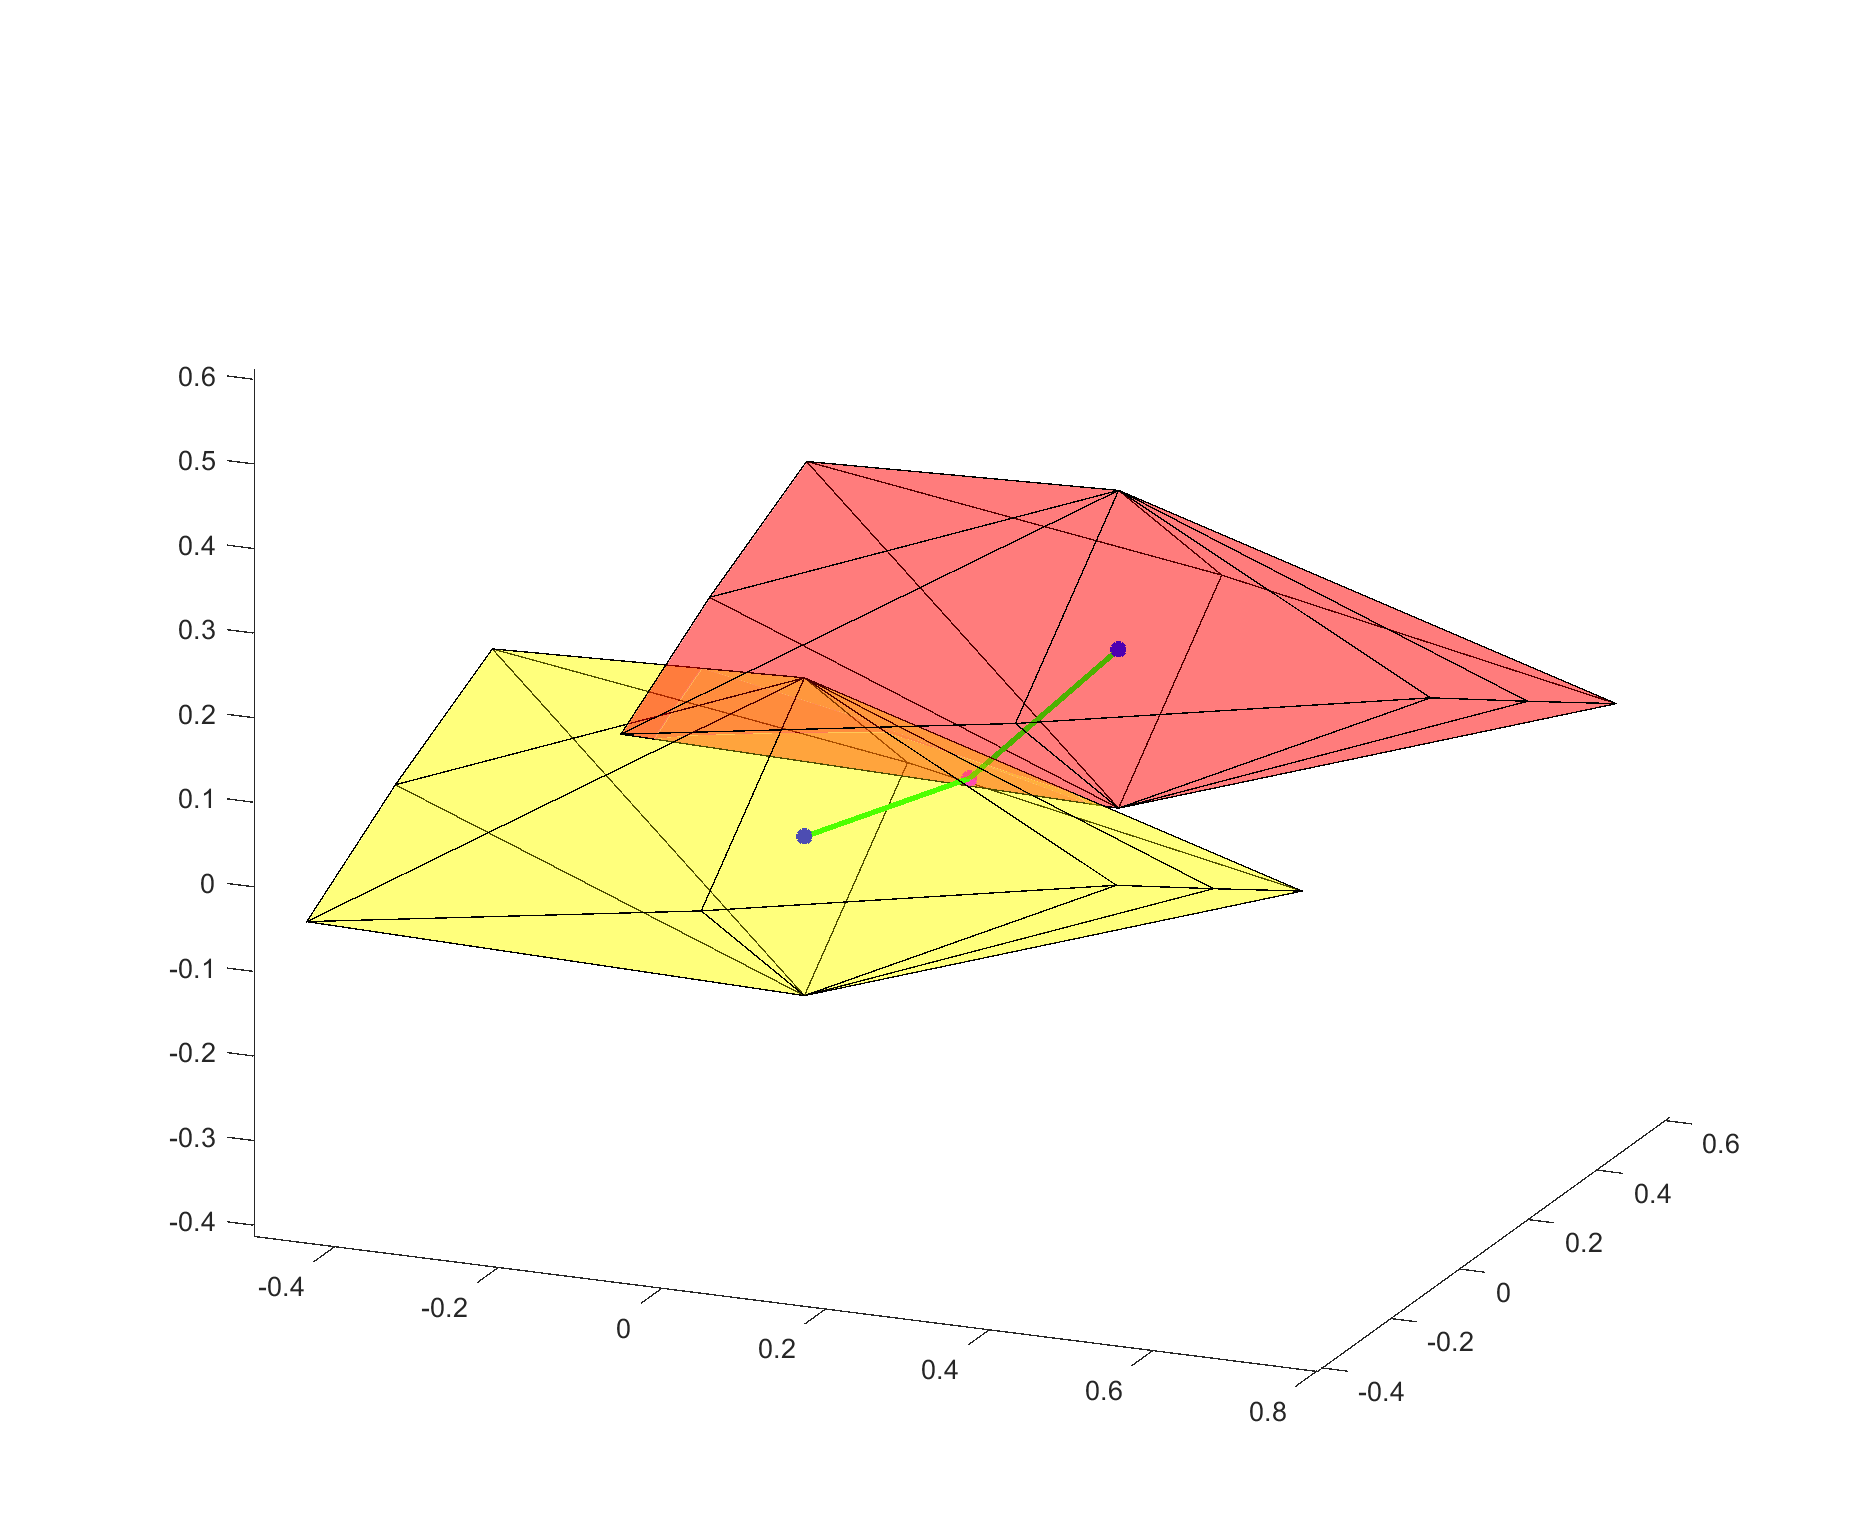
\includegraphics[scale=0.15]{layer_connection_c-space_polyhedron_fit.png}
\caption{Valid middle vertex sample and connections with vertices in different layers}
\label{fig:c-space-fitted-midVtx-poly}
\end{figure}
\end{enumerate}

\item {\bf Add middle vertex to the roadmap}\\
The next step is to append the found middle vertex to the roadmap. It is found that if we append the middle vertex each time when we found it, the time to re-allocate the memory of the vertex array and adjacency matrix is long. So for faster process, we need to pre-allocate the Vertex array and Adjacency matrix by doubling the memory before the ``for loops'' to find the middle vertices.

\item {\bf Results in Euclidean space}\\
Fig \ref{fig:eu-space} shows the result in Euclidean space, where there are two vertices, and the black ones are larger ellipses, the blue ones are smaller ellipses, and the red one is the connected middle vertex.

\begin{figure}[h]
\centering
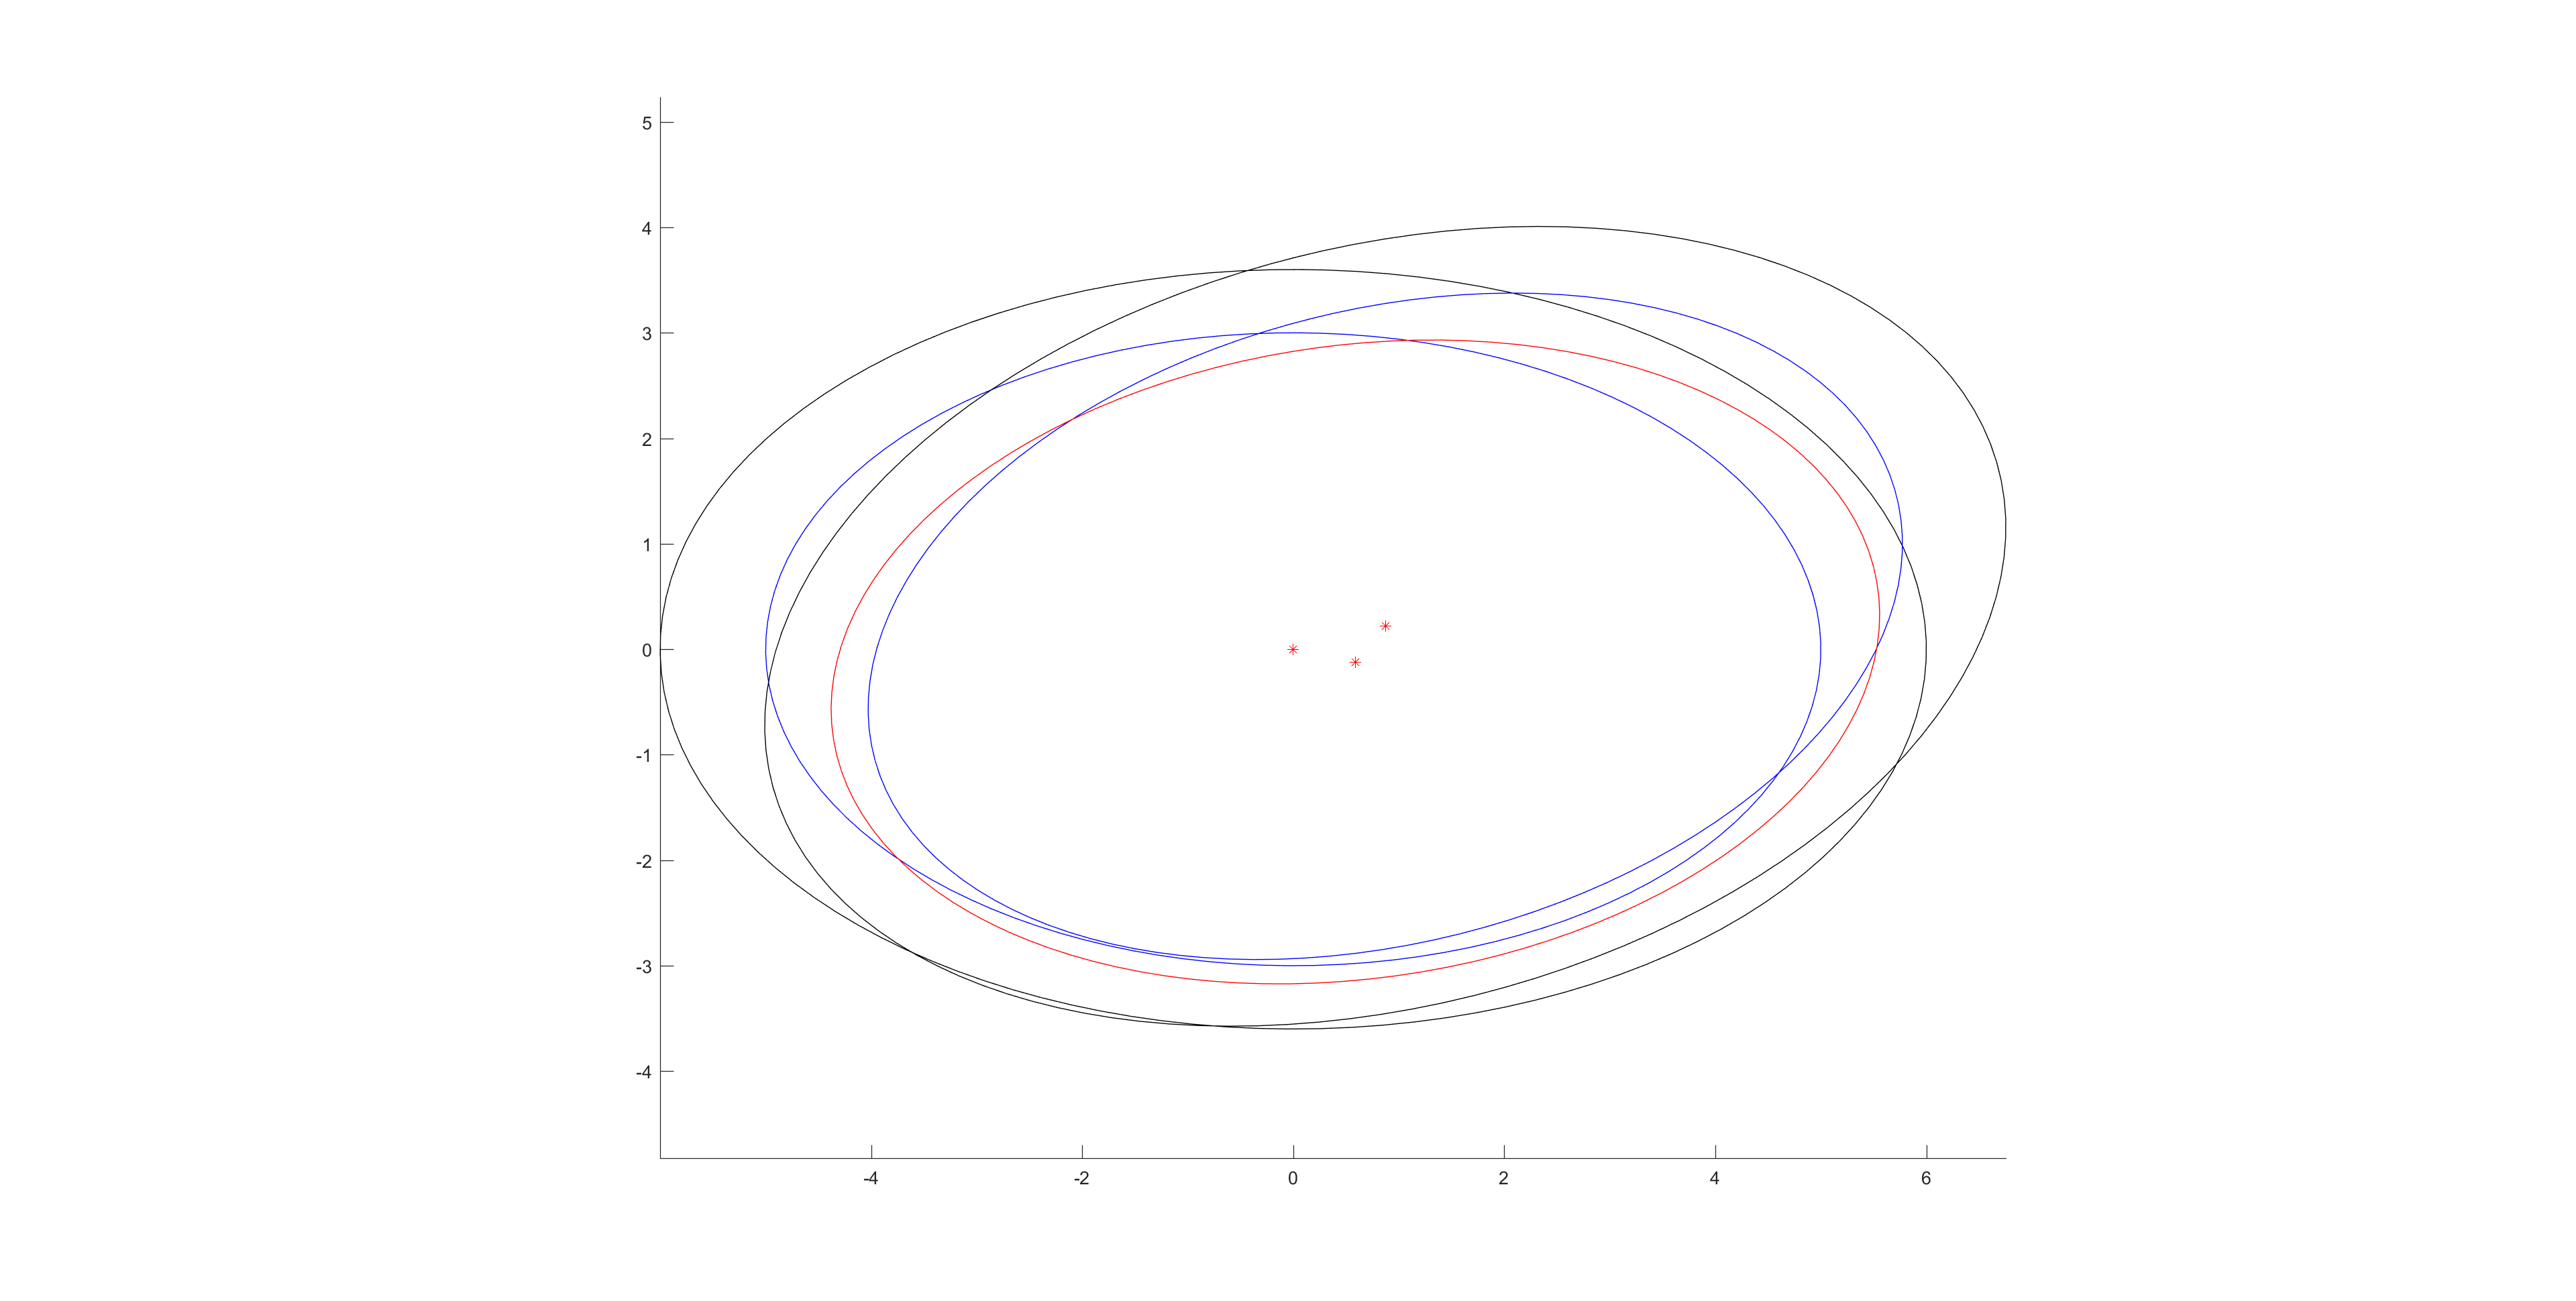
\includegraphics[scale=0.15]{layer_connection_euclidean_space.png}
\caption{Results in Euclidean space}
\label{fig:eu-space}
\end{figure}

\end{enumerate}

%%%% More ideas about connection layers
\item {\bf More ideas about connecting vertices in different layers}\\
Apart from generating a middle point, we could also directly connect two points. One direct way is to test whether one vertex is inside the local c-space of the other. This might be a strict condition, which in most cases might not return a valid result. Rather, we could generate points that are inside the local c-space instead of the sample-test process. Once we find the closest vertex $V_{i+1}$ in layer $i+1$ of the vertex $V_i$ in layer $i$, we could know the line segment where  $V_{i+1}$ is on. The line segment can be parameterized as $L_{p_1,p_2} = \frac{p_1 + p_2}{2} + \frac{t^2-1}{t^2+1} \frac{p_1 - p_2}{2}$ where $t\in(-\infty,+\infty)$ and $p = [x,y,\theta]^T$. So for the case of polyhedron fit, if we plug the parameterized line into the linear system of equations related to the only variable $t$, the problem becomes finding roots $t$ such that the values of the quadratic functions fall in the range of $[0,1]$. In such case, we could directly find valid points on the sweep line in layer $i+1$ which fall inside the local c-space of $V_i$. Since points along one sweep line can be connected safely, we could connect the newly found vertex with $V_i$ and $V_{i+1}$ respectively. We could also test more adjacent sweep lines that are close to $V_{i+1}$ to raise the possibility of finding valid points to connect. 

%%%% Determine the number of layers
\item {\bf Kinematics of Containment: a way to determine the number of layers and connect vertices between layers safely}\\
Another essential issue if to connect vertices between different layers. The goal is to find a safe way to connect with as small numbers of layers as possible. We tried to adopt the Kinematics of Containment (KC) method to fulfill it.

\begin{enumerate}
\item Condition of connectivity with vertices between different layers\\
We first explode the actual ellipsoid a little bit (i.e. scale = 1.1). For different layers, we fix translation part of the motion ({\bf Maybe could add some threshold $\epsilon$ to restrict the position within a range}), and only consider rotations of the exploded ellipsoids ($E_{EXPi}$ and $E_{EXPi+1}$ for exploded ellipsoids in $i$th and $i+1$th layers respectively). Since the distance between two layers are fixed (i.e. in 2D case, the rotational angle difference between two adjacent layers is fixed), we only consider the connectivity between adjacent layers. And our goal is to find the maximum layer distance such that there exist two actual ellipsoids ($E_i$ and $E_{i+1}$ for $i$th and $i+1$th layer) in different layers respectively that have the same configuration (i.e. same rotation angle and position) as seen in the world frame. We adjust the number of layers in order to change the distance between two layers since they are related.
	
\begin{figure}
\centering
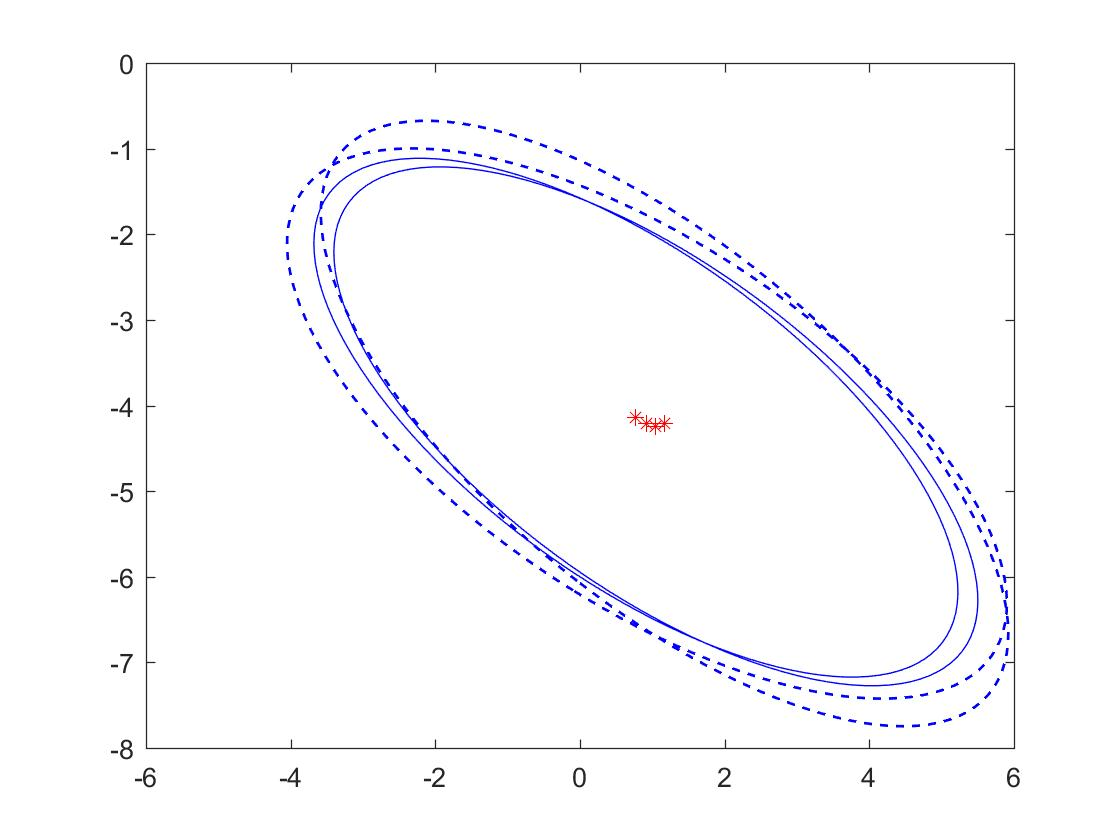
\includegraphics[scale = 0.2]{KC.jpg}
\caption{Condition judged by Kinematics of Containment.}
\label{fig:KC}
\end{figure}
	
We initialize a layer number $N$, and calculate the layer distance accordingly. Then,  using closed-form KC algorithm with ``direct sampling'' method, we sample 50 relative configurations of actual ellipsoids inside the exploded ellipsoids $E_{EXPi}$ and $E_{EXPi+1}$ respectively. We further calculate the configuration with respect to the world frame for those samples, and compare each pair from different layers. The procedure will keep going with the number of layers added and the layer distance decreased until the two samples with same configuration $C$ are found ({\bf we need to record the configuration also, and should add them into the vertices and adjacent matrix}). By this mean, we could not only determine that the two adjacent layers can be safely connected at configuration $C$, but also find the minimum number of layers, and thus decrease the number of vertices that needed to construct the roadmap.
	
\item Results of connections\\
The above searching process gives us a priori for the connectivity between different layers. With this knowledge, during the planning procedure, we could first generate C-space roadmap with the exploded ellipsoid for a single layer. And for connections between different layers, we just search for vertices in adjacent layers that are close to each other (the Euclidean distance of the center point of two vertices are close enough, which is in the range of $\epsilon$). The prior knowledge shows there exist a configuration $C$ for the actual ellipsoid that can be encapsulated within both exploded ellipsoids, we can simply connect these two vertices and ensure the actual ellipsoid moves in the free space (i.e In $i$th layer, $E_i$ aligns with $E_{EXPi}$; While moving to $i+1$th layer, if $E_{EXPi+1}$ is close to $E_{EXPi}$, $E_i$ could just move to configuration $C$ inside $E_{EXPi}$, then it could transfer into $E_{EXPi+1}$ safely; further, it could move to be aligned with $E_{EXPi+1}$ in $i+1$th layer).
	
\begin{figure}
\centering
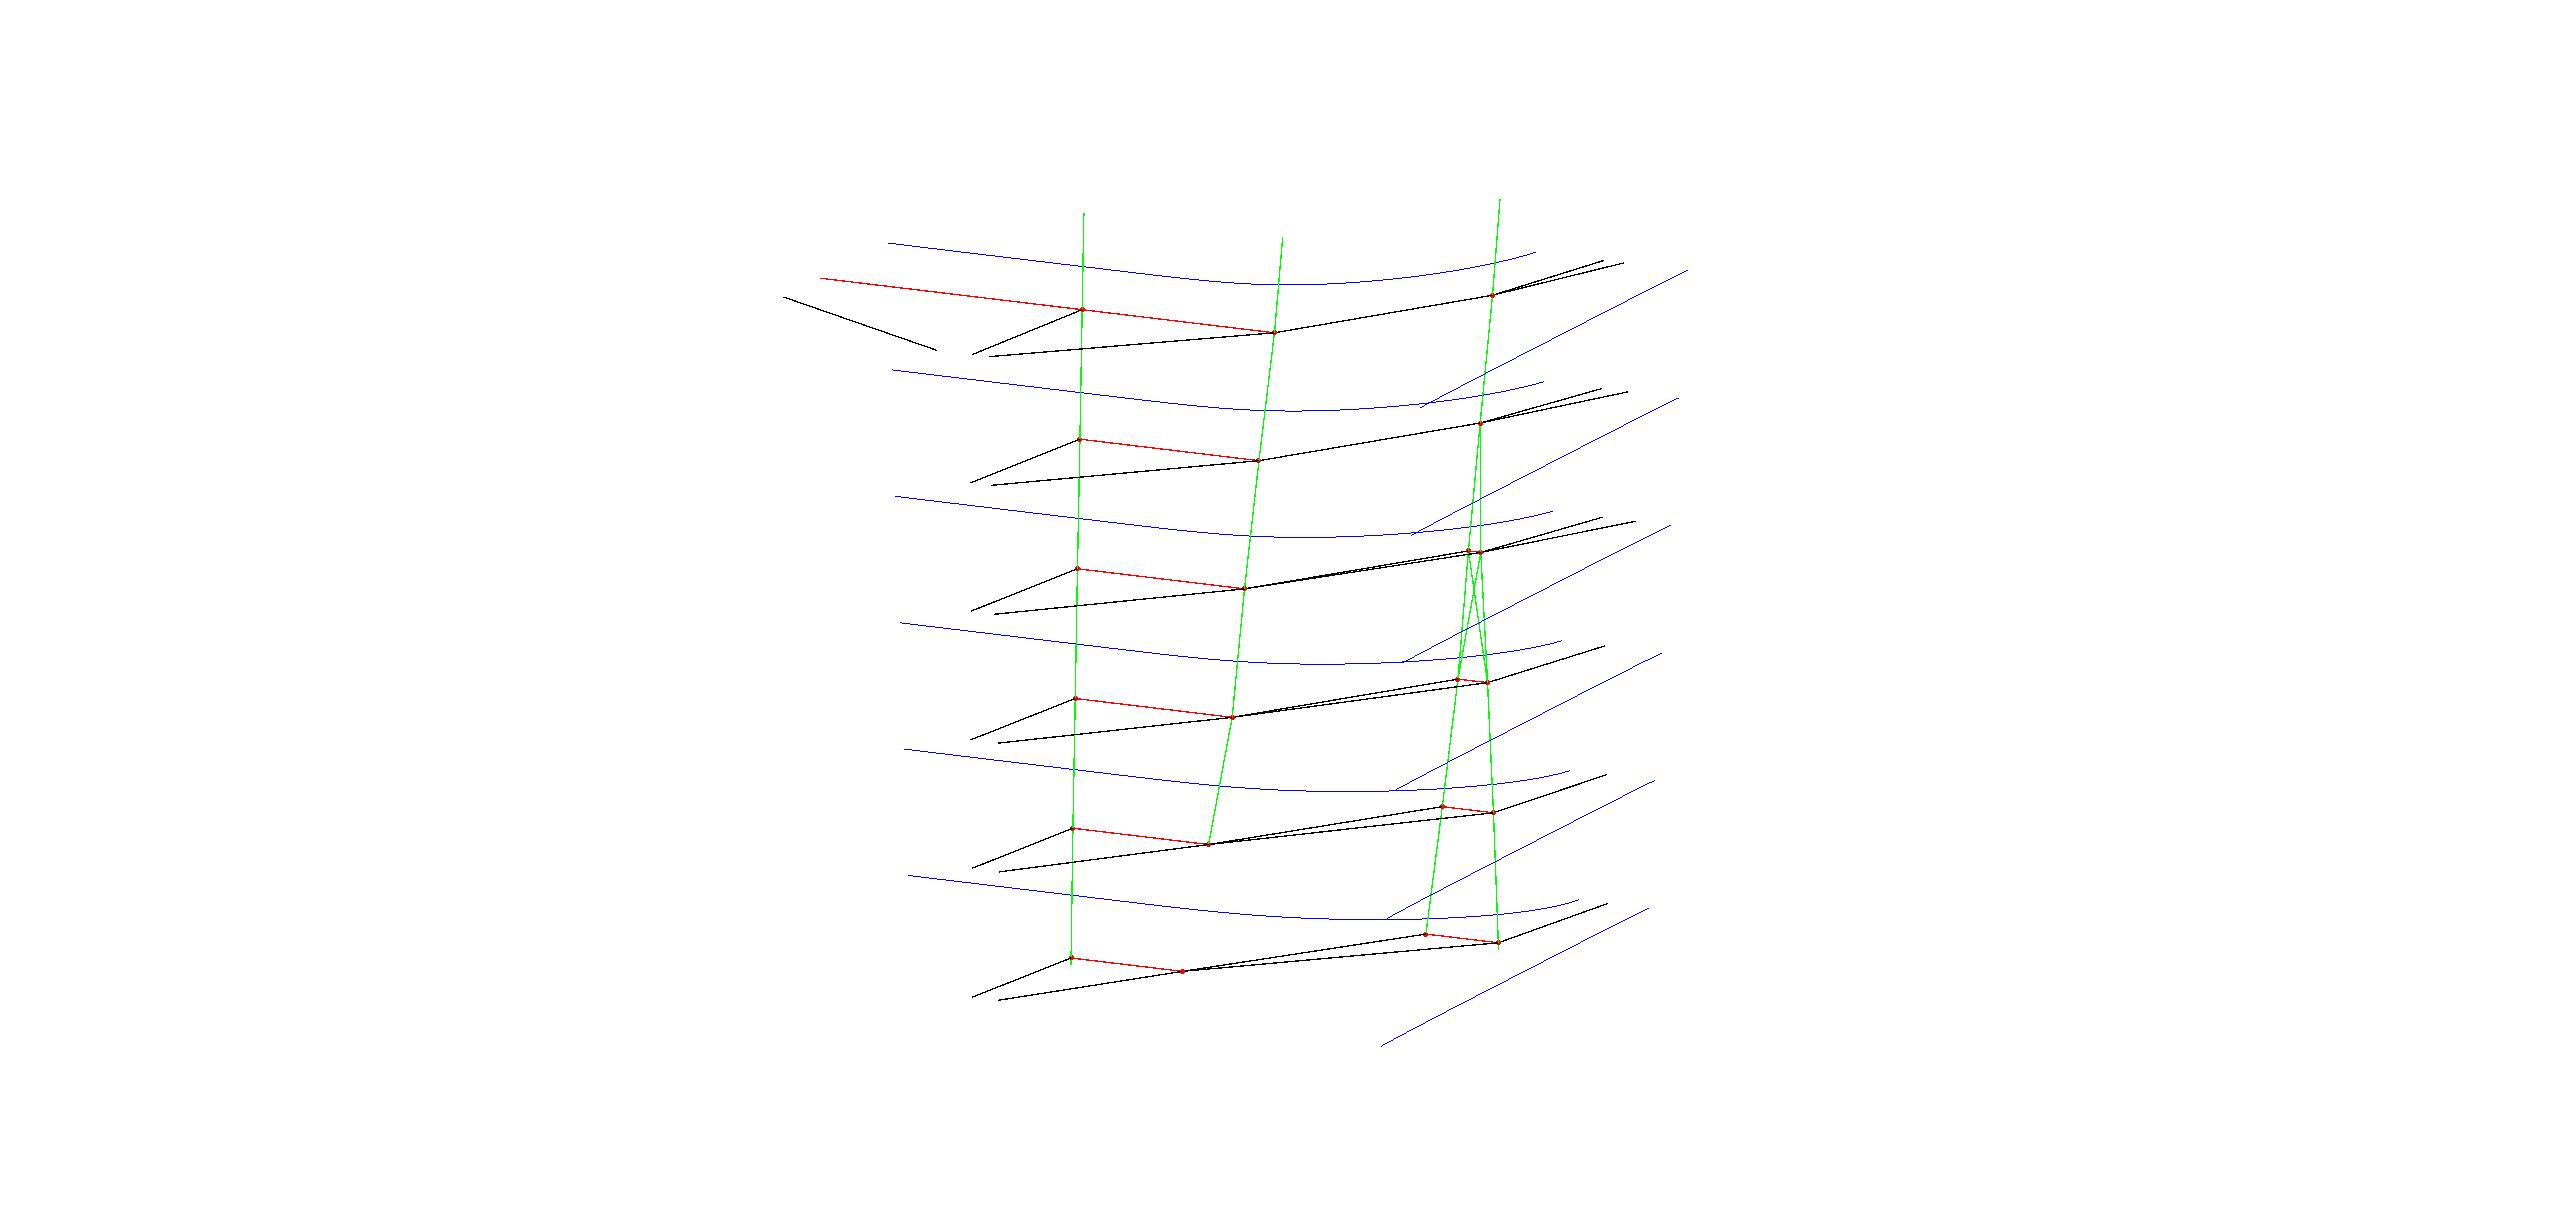
\includegraphics[scale = 0.2]{layerConnection_zoomIn.jpg}
\caption{Details of vertex connections. Green: connections between different layers.}
\label{fig:path_zoomIn}
\end{figure}
	
\begin{figure}
\centering
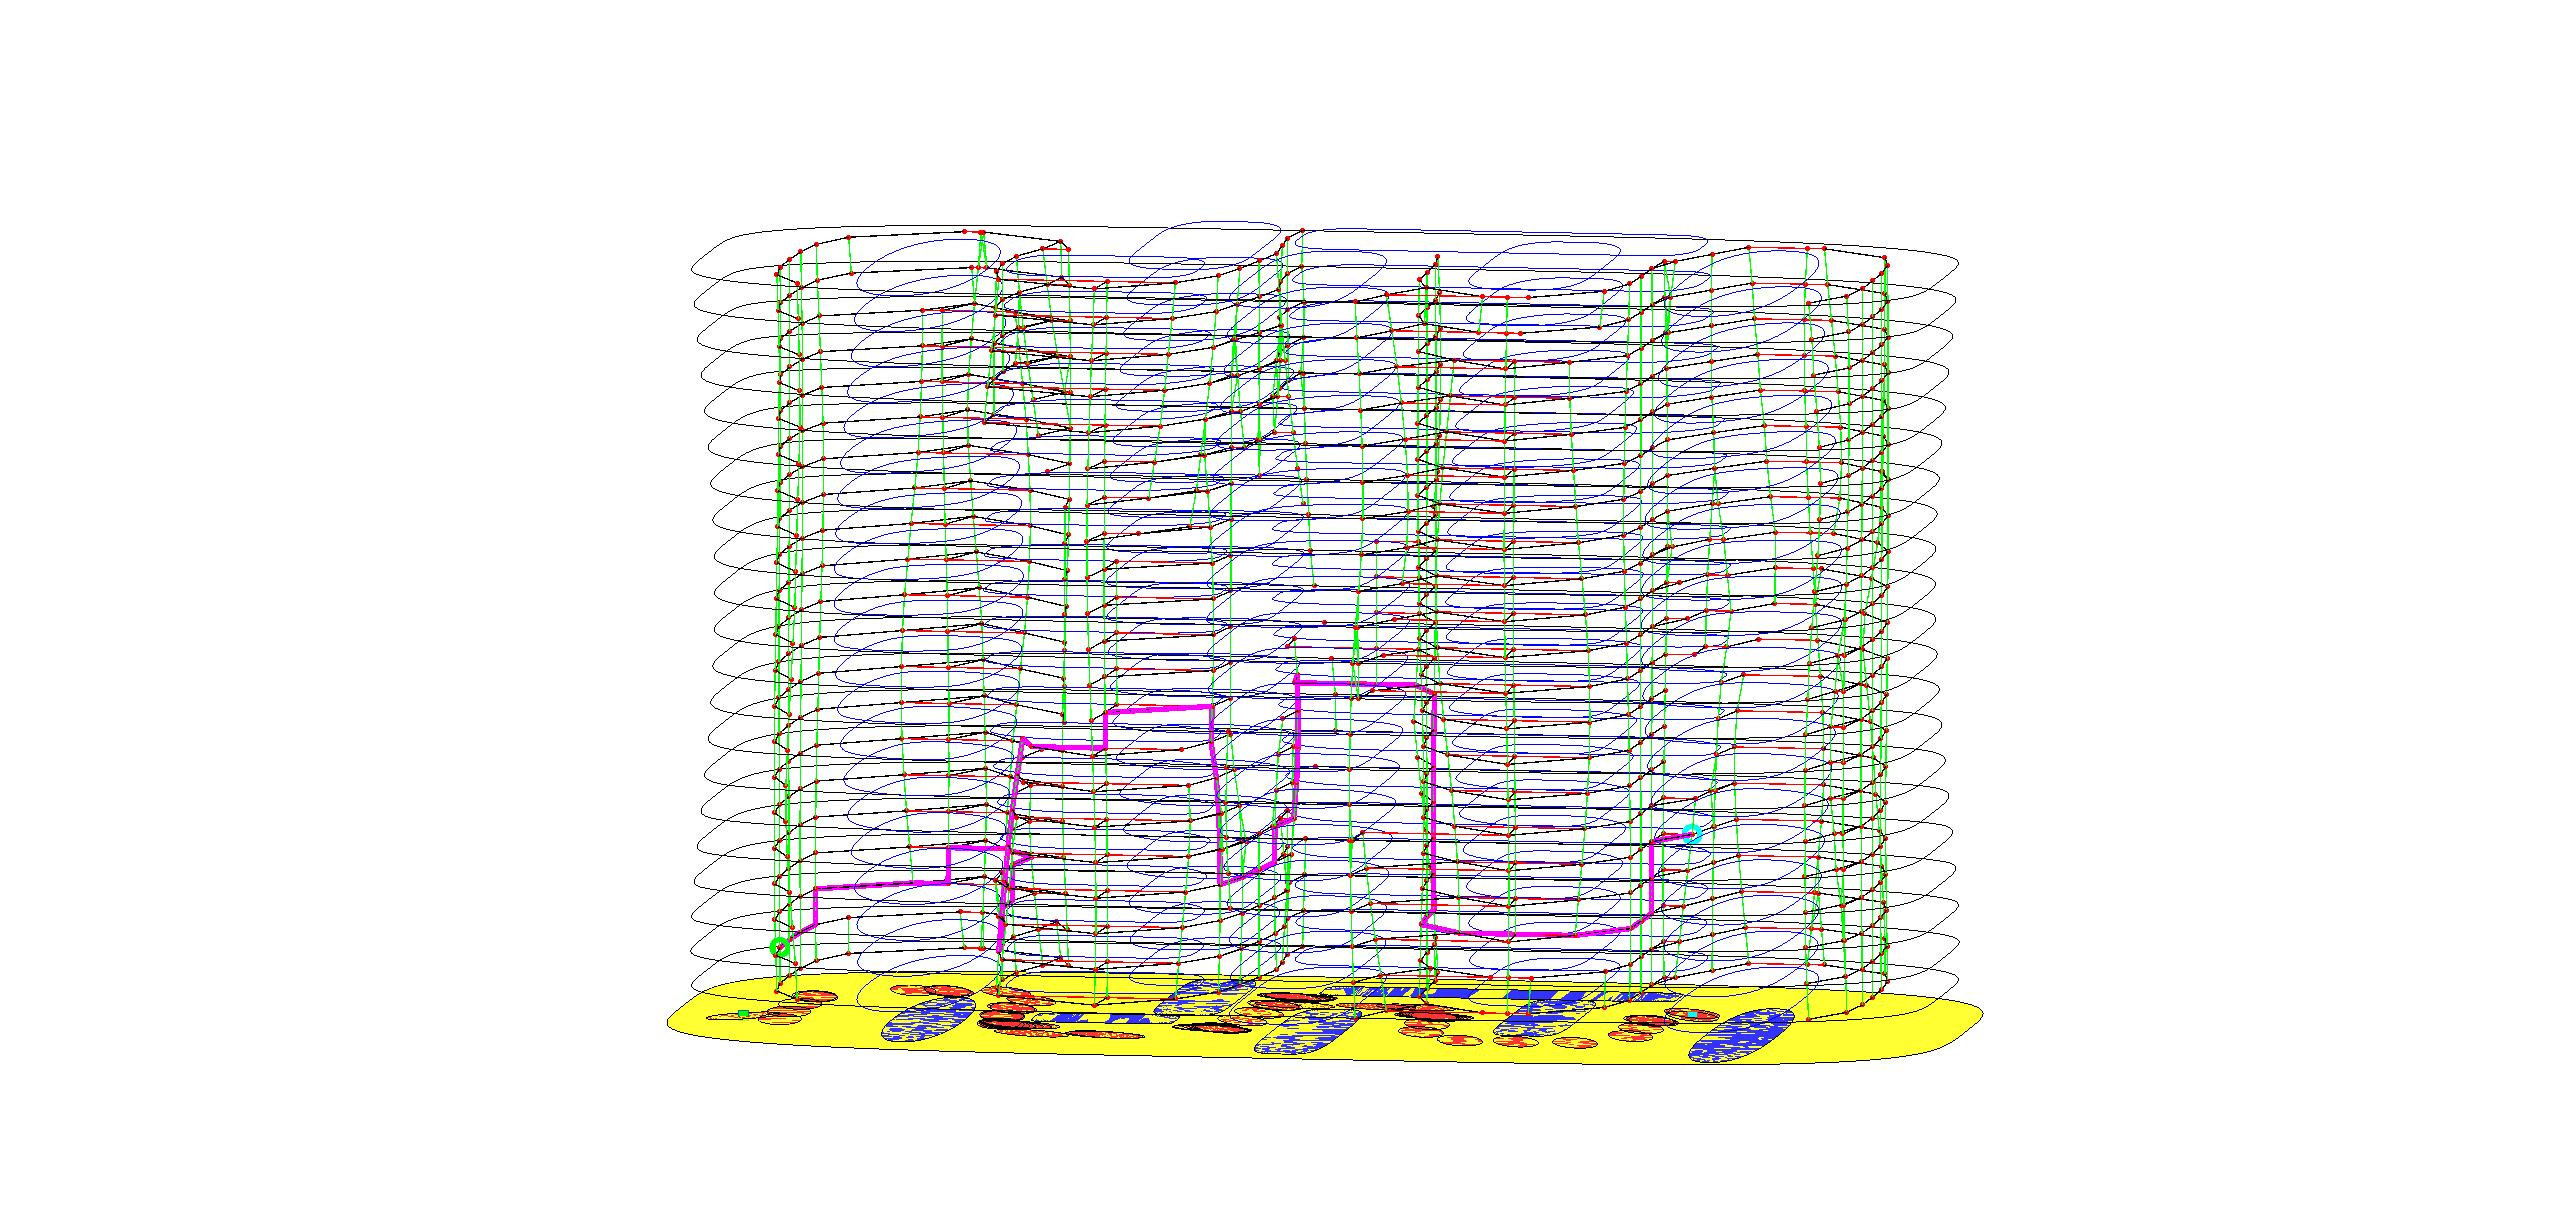
\includegraphics[scale = 0.2]{path_3d.jpg}
\label{fig:path_3d}
\caption{Highway Roadmap}
\end{figure}
	
\end{enumerate}

\end{enumerate}
\end{document}
